\question{Твердотельные лазеры. Рубиновый лазер.}
Генерация происходит в импульсном режиме на переходах между метастабильным
возбужденным и основным состояниями ионов \( Cr^{3+} \) на волне около
\( 0,69~\text{мкм} \). Инверсия достигается по трехуровневой схеме оптической
накачки, что является характерной чертой рубинового лазера. Излучение
немонохроматичной лампы-вспышки эффективно поглощается на переходах из
основного состояния хрома \term{4}{A}{2} в широкие полосы
\term{4}{F}{2} и \term{4}{F}{1}.

\begin{figure}[h]
    \center
    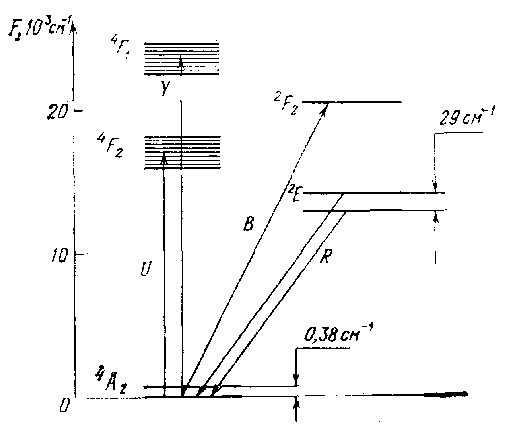
\includegraphics[width=.47\textwidth]{16}
    \caption{Уровни энергии рубина}
\end{figure}

На резонансных уровнях \term{4}{F}{1} и \term{4}{F}{2} энергия возбуждения не
накапливается и быстро безызлучательно переходит на метастабильное состояние
\term{4}{E}{}, населенность которого достигается засчет сравнительно большого
времени жизни этого состояния.

Для получения инверсии необходима предварительная затрата энергии, что в
трехуровневой схеме рубина обусловлено необходимостью перевести в метастабильное
состояние по крайней мере половину всех частиц.

Рубиновые лазеры обладают высокими энергетическими параметрами:
\begin{center}
    \begin{tabular}{|c|c|} \hline
        Поглощение в полосах накачки & \( 2-3~\text{см}^{-1} \) \\
        Пороговое значение энергии накачки &
            \( 3~\frac{\text{Дж}}{\text{см}^{3}} \) \\
        Объёмная плотность энергии в импульсах &
            \( 0,2-0,25~\frac{\text{Дж}}{\text{см}^{3}} \) \\
        Коэффициент линейного усиления & \( 0,2-0,25~\text{см}^{-1} \) \\
        \hline
    \end{tabular}
\end{center}

Возможны также импульсно-периодический и (для высококачественных кристаллов)
непрерывный режимы работы.

